\documentclass[aspectratio=169,11pt]{beamer}
\usetheme{Madrid}
\usecolortheme{default}

% Fix navigation symbols overflow in 16:9
\setbeamertemplate{navigation symbols}{}
\setbeamertemplate{footline}{
    \leavevmode%
    \hbox{%
        \begin{beamercolorbox}[wd=.333333\paperwidth,ht=2.25ex,dp=1ex,center]{author in head/foot}%
            \usebeamerfont{author in head/foot}\insertshortauthor
        \end{beamercolorbox}%
        \begin{beamercolorbox}[wd=.333333\paperwidth,ht=2.25ex,dp=1ex,center]{title in head/foot}%
            \usebeamerfont{title in head/foot}\insertshorttitle
        \end{beamercolorbox}%
        \begin{beamercolorbox}[wd=.333333\paperwidth,ht=2.25ex,dp=1ex,right]{date in head/foot}%
            \usebeamerfont{date in head/foot}\insertshortdate{}\hspace*{2em}
            \insertframenumber{} / \inserttotalframenumber\hspace*{2ex}
        \end{beamercolorbox}}%
    \vskip0pt%
}

% Custom colors
\definecolor{privacyblue}{RGB}{0,82,147}
\definecolor{privacygold}{RGB}{218,165,32}
\definecolor{privacygreen}{RGB}{34,139,34}
\definecolor{privacyred}{RGB}{178,34,34}
\definecolor{privacypurple}{RGB}{102,51,153}

\setbeamercolor{structure}{fg=privacyblue}
\setbeamercolor{title}{fg=white,bg=privacyblue}
\setbeamercolor{frametitle}{fg=white,bg=privacyblue}
\setbeamercolor{block title}{fg=white,bg=privacyblue}
\setbeamercolor{block body}{bg=privacyblue!10}

% Packages
\usepackage{tikz}
\usetikzlibrary{shapes,arrows,positioning,decorations.pathreplacing,calc}
\usepackage{booktabs}
\usepackage{tcolorbox}
\tcbuselibrary{skins,breakable}

% Custom boxes
\newtcolorbox{conceptbox}[1][]{
    colback=privacyblue!5,
    colframe=privacyblue,
    fonttitle=\bfseries,
    title=#1
}

\newtcolorbox{probox}[1][]{
    colback=privacygreen!5,
    colframe=privacygreen!80!black,
    fonttitle=\bfseries,
    title=#1
}

\newtcolorbox{objectionbox}[1][]{
    colback=privacyred!5,
    colframe=privacyred!80!black,
    fonttitle=\bfseries,
    title=#1
}

\newtcolorbox{casestudybox}[1][]{
    colback=privacygold!10,
    colframe=privacygold!80!black,
    fonttitle=\bfseries,
    title=#1
}

\newtcolorbox{quotebox}{
    colback=gray!10,
    colframe=gray!50,
    left=10pt,
    right=10pt,
    boxrule=0pt,
    leftrule=3pt
}

% Title information
\title[Privacy]{Privacy in the Information Age}
\subtitle{Surveillance, Data, and the Boundaries of the Self}
\author{Computing and AI Ethics}
\institute{Rochester Community and Technical College}
\date{}

\begin{document}

% Slide 1: Title
\begin{frame}
\titlepage
\end{frame}

% Slide 2: Central Questions
\begin{frame}{Central Questions}
\begin{itemize}
    \item What is privacy, and why does it matter?
    \item Do we have a ``right'' to privacy? If so, where does it come from?
    \item How has information technology transformed privacy?
    \item When (if ever) is surveillance justified?
    \item Is privacy a universal value, or culturally contingent?
\end{itemize}

\vspace{0.5em}
\begin{alertblock}{Discussion}
What's the last thing you did to protect your privacy online?
\end{alertblock}
\end{frame}

%% PART I: UNDERSTANDING PRIVACY %%
\section{Part I: Understanding Privacy}

% Slide 3: What Is Privacy?
\begin{frame}{What Is Privacy? Defining the Concept}
\begin{conceptbox}[Defining Privacy]
\small
Privacy is surprisingly difficult to define precisely:
\begin{itemize}
    \item ``The right to be let alone'' (Warren \& Brandeis, 1890)
    \item Control over information about oneself
    \item \textbf{Contextual integrity} (Helen Nissenbaum): Information flows appropriate to context
\end{itemize}
\end{conceptbox}

\vspace{0.3em}
\textbf{Key distinctions}: Privacy $\neq$ Secrecy $\neq$ Anonymity (related but distinct)

\textbf{Key insight}: Privacy is not about having something to hide---it's about maintaining boundaries between self and world.
\end{frame}

% Slide 4: Types of Privacy
\begin{frame}{Types of Privacy (Taxonomy)}
\begin{table}[h]
\centering
\scriptsize
\begin{tabular}{@{}llp{4cm}@{}}
\toprule
\textbf{Type} & \textbf{Description} & \textbf{Example Violation} \\
\midrule
\textbf{Informational} & Control over personal data & Data breach exposing records \\
\textbf{Physical/Spatial} & Freedom from bodily intrusion & Warrantless search \\
\textbf{Decisional} & Autonomy over personal choices & Reproductive restrictions \\
\textbf{Communications} & Private correspondence & Wiretapping \\
\textbf{Associational} & Freedom to associate privately & Membership list disclosure \\
\textbf{Intellectual} & Private thoughts and beliefs & Compelled speech \\
\bottomrule
\end{tabular}
\end{table}

\vspace{0.2em}
Different privacy types may require different protections.

\begin{alertblock}{Discussion}
Which type of privacy do you value most?
\end{alertblock}
\end{frame}

% Slide 5: Why Privacy Matters - Instrumental
\begin{frame}{Why Privacy Matters---Instrumental Arguments}
\begin{probox}[Privacy Serves Important Functions]
\scriptsize
\begin{enumerate}
    \item Privacy provides space for \textbf{autonomy}---room to develop our identities without external pressure.
    \item Selective sharing creates \textbf{intimacy}; we build relationships by choosing what to reveal.
    \item \textbf{Democracy} depends on privacy: anonymous ballots, confidential sources, and dissent.
    \item Privacy offers \textbf{security} against identity theft, stalking, and discrimination.
    \item It maintains \textbf{power balance}---asymmetric surveillance enables abuse.
\end{enumerate}
\end{probox}

\begin{quotebox}
\small
``Arguing that you don't care about privacy because you have nothing to hide is like arguing you don't care about free speech because you have nothing to say.'' \hfill---Edward Snowden
\end{quotebox}
\end{frame}

% Slide 6: Why Privacy Matters - Intrinsic
\begin{frame}{Why Privacy Matters---Intrinsic Arguments}
Privacy may have value \emph{beyond} its consequences:

\begin{columns}[T]
\begin{column}{0.55\textwidth}
\begin{itemize}
    \item Being observed without consent is degrading---privacy protects \textbf{dignity}.
    \item The ``self'' requires private boundaries; privacy is constitutive of \textbf{personhood}.
    \item Privacy acknowledges persons as ends, not means, expressing \textbf{respect}.
\end{itemize}

\vspace{0.3em}
\textbf{James Rachels}: Privacy enables us to maintain different relationships with different people.
\end{column}
\begin{column}{0.4\textwidth}
\begin{center}
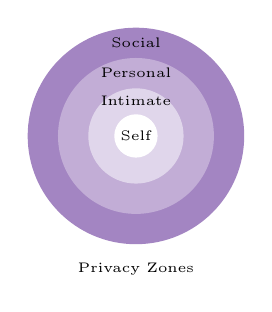
\begin{tikzpicture}[scale=0.55]
    \fill[privacypurple!60] (0,0) circle (2.5);
    \fill[privacypurple!40] (0,0) circle (1.8);
    \fill[privacypurple!20] (0,0) circle (1.1);
    \fill[white] (0,0) circle (0.5);
    \node[font=\tiny] at (0,0) {Self};
    \node[font=\tiny] at (0,0.8) {Intimate};
    \node[font=\tiny] at (0,1.45) {Personal};
    \node[font=\tiny] at (0,2.15) {Social};
    \node[font=\tiny, below] at (0,-2.7) {Privacy Zones};
\end{tikzpicture}
\end{center}
\end{column}
\end{columns}
\end{frame}

% Slide 7: Legal Foundations - US
\begin{frame}{Legal Foundations of Privacy---United States}
\begin{conceptbox}[US Privacy Law: A Patchwork Approach]
\small
\begin{itemize}
    \item \textbf{4th Amendment}: Protection against unreasonable searches
    \item \textbf{Griswold v. Connecticut} (1965): Privacy implied by ``penumbras''
    \item \textbf{Katz v. United States} (1967): ``Reasonable expectation of privacy''
    \item \textbf{Third-party doctrine}: Info shared with third parties loses protection
\end{itemize}
\end{conceptbox}

\vspace{0.2em}
\textbf{Sectoral approach}: HIPAA (health), GLBA (finance), COPPA (children), FERPA (education)

\textbf{Key gap}: \textbf{No comprehensive federal privacy law} (unlike EU)
\end{frame}

% Slide 8: Legal Foundations - International
\begin{frame}{Legal Foundations---International Comparison}
\begin{table}[h]
\centering
\scriptsize
\begin{tabular}{@{}llll@{}}
\toprule
\textbf{Jurisdiction} & \textbf{Approach} & \textbf{Key Law} & \textbf{Max Penalty} \\
\midrule
\textbf{EU} & Comprehensive right & GDPR (2018) & 4\% global revenue \\
\textbf{USA} & Sectoral, patchwork & Various (HIPAA, etc.) & Varies by sector \\
\textbf{China} & State control priority & PIPL (2021) & 5\% revenue \\
\textbf{California} & Consumer rights & CCPA/CPRA & \$7,500 per violation \\
\bottomrule
\end{tabular}
\end{table}

\vspace{0.2em}
\textbf{GDPR features}: Right to erasure, consent requirements, data portability

\textbf{Largest GDPR fine}: \texteuro1.2 billion to Meta (2023) for illegal data transfers

\begin{alertblock}{Discussion}
Should the US adopt GDPR-style comprehensive protections?
\end{alertblock}
\end{frame}

% Slide 9: Philosophical Theories
\begin{frame}{Philosophical Theories of Privacy Rights}
\begin{conceptbox}[Where Does the Right to Privacy Come From?]
\small
\begin{enumerate}
    \item \textbf{Natural rights}: Privacy inherent to human dignity (Kantian)
    \item \textbf{Utilitarian}: Privacy maximizes overall welfare
    \item \textbf{Social contract}: Privacy necessary for civil society
    \item \textbf{Property rights}: Personal data as property (Lockean)
    \item \textbf{Relational}: Privacy constitutes relationships (Rachels, Nissenbaum)
    \item \textbf{Feminist critique}: ``Personal is political''---privacy can hide abuse
\end{enumerate}
\end{conceptbox}

\vspace{0.2em}
\textbf{Key tension}: Privacy as \emph{protection} vs. privacy as \emph{concealment}
\end{frame}

% Slide 10: Skeptical Views of Privacy - Thomson
\begin{frame}{Skeptical Views: Is Privacy a Distinct Right?}
\begin{conceptbox}[Judith Jarvis Thomson's Reductionist Challenge (1975)]
\small
Thomson argued that ``privacy'' is not a distinct right at all---it can be fully explained by other rights we already recognize.
\end{conceptbox}

\vspace{0.1em}
\textbf{The argument in standard form}:
\begin{enumerate}
    \item Every privacy violation can be redescribed as a violation of property rights (entering your home) or bodily rights (touching you without consent).
    \item If privacy violations are always also violations of these other rights, privacy adds nothing new.
    \item Therefore, ``privacy'' is just a cluster concept, not a distinct right.
\end{enumerate}

\vspace{0.1em}
{\small \textbf{Response}: Critics argue Thomson misses cases where no property or bodily right is violated---such as watching you through a telephoto lens from public property, or aggregating your public data into a profile.}
\end{frame}

% Slide 11: Skeptical Views - Posner
\begin{frame}{Skeptical Views: The Economic Critique}
\begin{objectionbox}[Richard Posner's Economic Argument (1978)]
\small
Posner argued that privacy is often economically inefficient because it enables people to conceal information others have legitimate interests in knowing.
\end{objectionbox}

\vspace{0.1em}
\textbf{The argument in standard form}:
\begin{enumerate}
    \item Efficient markets require accurate information about participants.
    \item Privacy allows people to hide negative information (health conditions, past behavior, debts).
    \item Such concealment distorts decisions and creates inefficiencies.
    \item Therefore, strong privacy protections impose social costs.
\end{enumerate}

\vspace{0.1em}
{\small \textbf{Response}: This view treats people as mere economic actors and ignores power imbalances---the employer learns everything about you; you learn little about them. Privacy can \emph{correct} market failures by preventing irrelevant discrimination.}
\end{frame}

% Slide 12: Nothing to Hide Argument
\begin{frame}{The ``Nothing to Hide'' Argument}
\textbf{Common claim}: ``If you have nothing to hide, you have nothing to fear''

\begin{objectionbox}[Responses to ``Nothing to Hide'']
\small
\begin{enumerate}
    \item Everyone has something to hide (legal but private matters)
    \item Innocence doesn't guarantee safety (false positives, changed laws)
    \item \textbf{Chilling effects} on speech and behavior
    \item Power asymmetry: ``You show me yours first''
    \item \textbf{Aggregation problem}: Innocuous data combines into sensitive profiles
    \item Future unknown: Today's normal may be tomorrow's suspicious
\end{enumerate}
\end{objectionbox}

\vspace{0.2em}
\textbf{Daniel Solove}: The problem isn't isolated data, but the ``aggregation problem.''
\end{frame}

% Slide 13: Privacy Paradox
\begin{frame}{The Privacy Paradox}
\begin{conceptbox}[The Paradox]
People say they value privacy but act as if they don't.
\end{conceptbox}

\vspace{0.2em}
\textbf{Evidence}: Studies show high stated concern, yet people readily share data for small conveniences.

\textbf{Possible explanations}:
\begin{itemize}
    \item Privacy decisions are too complex to evaluate rationally (\textbf{bounded rationality})
    \item We favor immediate gratification over abstract future harm (\textbf{temporal discounting})
    \item Many feel resigned: ``Privacy is dead anyway''
    \item Often there's no real alternative---take it or leave it
\end{itemize}

\begin{alertblock}{Discussion}
Do your privacy behaviors match your stated privacy preferences?
\end{alertblock}
\end{frame}

% Slide 14: Case Study - Right to Be Forgotten
\begin{frame}{Case Study: The ``Right to Be Forgotten''}
\begin{casestudybox}[Google Spain v. AEPD (2014)]
\small
\textbf{Mario Costeja Gonz\'alez}: Wanted old newspaper links about debt removed from Google search results.\\
\textbf{EU Court ruling}: Individuals can request removal of ``inadequate, irrelevant, or excessive'' information.
\end{casestudybox}

\vspace{0.2em}
\textbf{Now in GDPR Article 17}: The ``right to erasure''

\textbf{Scale}: Google has received \textbf{2+ million removal requests} since 2014

\textbf{Tensions}: This ruling pits privacy against free speech and press freedom, and raises questions about memory versus forgetting in the digital age. The EU and US take fundamentally different approaches.

\begin{alertblock}{Discussion}
Should people be able to erase their digital past?
\end{alertblock}
\end{frame}

%% PART II: HISTORY OF IT AND PRIVACY %%
\section{Part II: A History of IT and Privacy}

% Slide 13: Pre-Digital Privacy
\begin{frame}{Pre-Digital Privacy Concerns}
Privacy concerns predate computers:

\begin{itemize}
    \item \textbf{1890}: Warren \& Brandeis ``The Right to Privacy''---response to photography and tabloid journalism
    \item \textbf{1928}: \emph{Olmstead v. United States}---wiretapping (Brandeis dissent)
    \item \textbf{1949}: Orwell's \emph{1984}---totalitarian surveillance state
    \item \textbf{1960s}: Government databases spark concern (Social Security numbers)
    \item \textbf{1970}: Fair Credit Reporting Act---first major US data privacy law
    \item \textbf{1974}: Privacy Act---governs federal agency records
\end{itemize}

\vspace{0.3em}
\textbf{Key insight}: Each new technology triggers new privacy concerns.
\end{frame}

% Slide 14: Computer Revolution
\begin{frame}{The Computer Revolution (1970s--1980s)}
\begin{center}
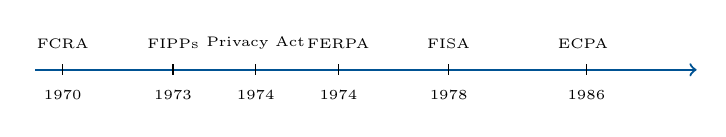
\begin{tikzpicture}[scale=0.7, every node/.style={font=\tiny}]
    \draw[thick, ->, privacyblue] (0,0) -- (12,0);
    \foreach \x/\year/\event in {
        0.5/1970/FCRA,
        2.5/1973/FIPPs,
        4/1974/Privacy Act,
        5.5/1974/FERPA,
        7.5/1978/FISA,
        10/1986/ECPA
    } {
        \draw (\x,0.1) -- (\x,-0.1);
        \node[above, align=center] at (\x,0.2) {\event};
        \node[below] at (\x,-0.2) {\year};
    }
\end{tikzpicture}
\end{center}

\vspace{0.3em}
\textbf{1973 HEW Report}: Established \textbf{Fair Information Practice Principles} (FIPPs):
\begin{itemize}
    \item Notice, Choice, Access, Security, Enforcement
\end{itemize}

\textbf{1978 FISA}: Created secret court for surveillance warrants

\textbf{1986 ECPA problem}: Stored communications $>$180 days get less protection (outdated assumption)
\end{frame}

% Slide 15: Internet Age
\begin{frame}{The Internet Age (1990s--2000s)}
\begin{itemize}
    \item \textbf{1991}: World Wide Web transforms information sharing
    \item \textbf{1995}: EU Data Protection Directive---comprehensive approach
    \item \textbf{1998}: COPPA---children's online privacy
    \item \textbf{1999}: Gramm-Leach-Bliley Act---financial privacy
    \item \textbf{2001}: USA PATRIOT Act---expands surveillance post-9/11
    \begin{itemize}
        \item Section 215: Bulk collection of phone metadata
        \item National Security Letters without judicial oversight
    \end{itemize}
\end{itemize}

\vspace{0.3em}
\textbf{New technologies emerge}: Cookies, web tracking, behavioral advertising
\end{frame}

% Slide 16: Social Media Era
\begin{frame}{The Social Media Era (2004--2012)}
\begin{columns}[T]
\begin{column}{0.55\textwidth}
\begin{itemize}
    \item \textbf{2004}: Facebook launches
    \item \textbf{2006}: Twitter; Facebook goes public
    \item \textbf{2007}: iPhone---smartphones ubiquitous
    \item \textbf{2010}: Facebook privacy policy controversies
    \item \textbf{2011}: Location tracking scandals
\end{itemize}

\vspace{0.3em}
\textbf{Business model}: ``If it's free, you're the product''
\end{column}
\begin{column}{0.42\textwidth}
\begin{table}[h]
\centering
\scriptsize
\begin{tabular}{@{}ll@{}}
\toprule
\textbf{Platform} & \textbf{Data Types} \\
\midrule
Facebook & Posts, location, contacts \\
Google & Searches, emails, YouTube \\
Amazon & Purchases, Alexa, browsing \\
\bottomrule
\end{tabular}
\caption*{\scriptsize Data collected (indefinite retention)}
\end{table}
\end{column}
\end{columns}
\end{frame}

% Slide 17: Snowden Revelations
\begin{frame}{Case Study: The Snowden Revelations (2013)}
\begin{casestudybox}[Edward Snowden: NSA Contractor Turned Whistleblower]
\small
\textbf{Key revelations}:
\begin{itemize}
    \item \textbf{PRISM}: Direct access to tech company servers
    \item \textbf{Upstream collection}: Tapping fiber optic cables
    \item \textbf{Bulk phone metadata}: Section 215 collection
    \item \textbf{XKeyscore}: ``Nearly everything a user does on the Internet''
\end{itemize}
\end{casestudybox}

\vspace{0.2em}
\textbf{Impact}: Global debate, USA FREEDOM Act (2015), encryption push

\textbf{Current status}: Snowden received Russian citizenship (2022), remains in Russia

\textbf{Ongoing debate}: Hero or traitor?
\end{frame}

% Slide 18: Cambridge Analytica
\begin{frame}{Case Study: Cambridge Analytica (2018)}
\begin{casestudybox}[The Data Harvesting Scandal]
\small
\textbf{What happened}: Political consulting firm harvested \textbf{87 million} Facebook profiles via personality quiz app ``This Is Your Digital Life''---collected data from users AND their friends.\\
\textbf{Use}: Psychographic profiling for targeted political ads (Brexit, 2016 US election)
\end{casestudybox}

\vspace{0.2em}
\textbf{Consequences}:
\begin{itemize}
    \item Mark Zuckerberg testified before Congress.
    \item The FTC levied a \$5 billion fine---the largest ever for privacy at the time.
    \item The scandal accelerated GDPR implementation (May 2018).
    \item Public awareness of data practices increased dramatically.
\end{itemize}

\textbf{Lesson}: ``Move fast and break things'' meets democracy
\end{frame}

% Slide 19: Current Landscape
\begin{frame}{The Current Landscape (2020s)}
\begin{columns}[T]
\begin{column}{0.55\textwidth}
\textbf{New technologies}:
\begin{itemize}
    \item AI and machine learning power facial recognition and predictive systems.
    \item The Internet of Things puts sensors in our homes, on our bodies, and in our cars.
    \item Biometric identification now extends to faces, voices, and DNA.
    \item Generative AI systems train on vast troves of personal data.
\end{itemize}

\textbf{COVID-19 impact}: Contact tracing, health passports, remote work surveillance
\end{column}
\begin{column}{0.42\textwidth}
\begin{table}[h]
\centering
\scriptsize
\begin{tabular}{@{}lr@{}}
\toprule
\textbf{Data Broker Stats} & \\
\midrule
Market size (2024) & \$280B+ \\
Brokers globally & $\sim$5,000 \\
Avg databases/American & 1,500+ \\
Data points/profile & 1,500+ \\
\bottomrule
\end{tabular}
\end{table}
\end{column}
\end{columns}
\end{frame}

% Slide 20: Surveillance Capitalism
\begin{frame}{The Attention Economy and Surveillance Capitalism}
\begin{conceptbox}[Shoshana Zuboff's Framework (2019)]
\small
\begin{enumerate}
    \item \textbf{Human experience} as raw material for data extraction
    \item \textbf{Behavioral surplus}: Data beyond service improvement $\rightarrow$ prediction products
    \item \textbf{Prediction products} sold to business customers (advertisers)
    \item \textbf{Behavioral modification}: Nudging users toward desired outcomes
    \item \textbf{Instrumentarian power}: Shaping behavior at scale
\end{enumerate}
\end{conceptbox}

\vspace{0.2em}
\begin{quotebox}
\small
``Surveillance capitalism unilaterally claims human experience as free raw material for translation into behavioral data.''
\end{quotebox}
\end{frame}

%% PART III: SURVEILLANCE IN AUTHORITARIAN STATES %%
\section{Part III: IT Surveillance in Authoritarian States}

% Slide 21: Surveillance and Regime Type
\begin{frame}{Surveillance and Regime Type}
\begin{center}
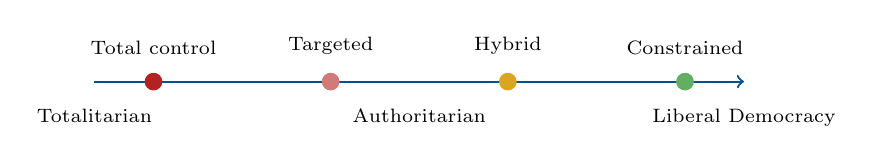
\begin{tikzpicture}[scale=0.75, every node/.style={font=\scriptsize}]
    \draw[thick, ->, privacyblue] (0,0) -- (11,0);
    \node[below] at (0,-0.3) {Totalitarian};
    \node[below] at (5.5,-0.3) {Authoritarian};
    \node[below] at (11,-0.3) {Liberal Democracy};
    
    \fill[privacyred] (1,0) circle (0.15);
    \node[above] at (1,0.3) {Total control};
    
    \fill[privacyred!60] (4,0) circle (0.15);
    \node[above] at (4,0.3) {Targeted};
    
    \fill[privacygold] (7,0) circle (0.15);
    \node[above] at (7,0.3) {Hybrid};
    
    \fill[privacygreen!70] (10,0) circle (0.15);
    \node[above] at (10,0.3) {Constrained};
\end{tikzpicture}
\end{center}

\vspace{0.3em}
\textbf{Key insight}: Technology has made comprehensive surveillance far cheaper and more effective than ever before.

\begin{alertblock}{Central Question}
Can liberal democracies use these technologies without becoming authoritarian?
\end{alertblock}
\end{frame}

% Slide 22: China Overview
\begin{frame}{China---The Surveillance State Model}
\begin{objectionbox}[The Most Comprehensive Surveillance System in History]
\small
\begin{itemize}
    \item \textbf{1.4 billion people}, world's largest population
    \item \textbf{Social Credit System}: Scoring citizens on ``trustworthiness''
    \item \textbf{600--700 million CCTV cameras} nationwide
    \item \textbf{Great Firewall}: Blocks Google, Facebook, Twitter, foreign news
    \item \textbf{Real-name registration}: Required for internet, phone, transit
\end{itemize}
\end{objectionbox}

\vspace{0.2em}
\vspace{0.2em}
\textbf{Social Credit consequences}:
\begin{itemize}
    \item High scores bring rewards like fast-track services and better loan rates.
    \item Low scores trigger punishments: travel bans, public shaming, and job restrictions.
\end{itemize}
\end{frame}

% Slide 23: China Facial Recognition
\begin{frame}{China---Facial Recognition and AI}
\begin{table}[h]
\centering
\scriptsize
\begin{tabular}{@{}llr@{}}
\toprule
\textbf{System} & \textbf{Function} & \textbf{Scale} \\
\midrule
Skynet/Sharp Eyes & Urban camera network & 600M+ cameras \\
Golden Shield & Database integration & 1.4B citizens \\
Great Firewall & Internet censorship & All traffic \\
Social Credit & Behavior scoring & National \\
\bottomrule
\end{tabular}
\end{table}

\vspace{0.2em}
\textbf{AI capabilities}:
\begin{itemize}
    \item These systems can identify faces in crowds and track individuals across cities.
    \item Some claim to detect suspicious behavior through ``emotion recognition'' and gait recognition---though the science is dubious.
    \item Integration of cameras with phones, apps, and payments creates comprehensive tracking.
\end{itemize}

\textbf{Tech exporters}: Huawei, Hikvision, SenseTime, Megvii
\end{frame}

% Slide 24: Xinjiang Uyghurs
\begin{frame}{Case Study: Xinjiang and the Uyghurs}
\begin{casestudybox}[Surveillance-Enabled Persecution]
\small
\textbf{Xinjiang Uyghur Autonomous Region}: $\sim$12 million Uyghur Muslims\\
\textbf{Mass detention}: 1+ million detained in ``re-education camps'' (2017--present); $\sim$500,000 currently in prisons/detention (2025 estimate)
\end{casestudybox}

\vspace{0.2em}
\textbf{Surveillance intensity}:
\begin{itemize}
    \item In some areas, checkpoints appear every 100 meters.
    \item Residents must install mandatory smartphone apps and submit to DNA collection.
    \item The IJOP predictive system flags ``suspicious'' behaviors---including praying, traveling abroad, or having certain contacts.
\end{itemize}

\textbf{International response}: US sanctions on Hikvision, genocide determinations by US, UK, Canada, EU Parliament

\textbf{Lesson}: Technology enables persecution at unprecedented scale
\end{frame}

% Slide 25: Russia
\begin{frame}{Russia---Selective Surveillance and SORM}
\begin{conceptbox}[SORM: System of Operative-Investigative Measures]
\small
\begin{itemize}
    \item Requires ISPs to install FSB monitoring equipment
    \item Real-time access \textbf{without judicial warrant}
    \item SORM-1 (phones), SORM-2 (internet), SORM-3 (all communications)
\end{itemize}
\end{conceptbox}

\vspace{0.2em}
Russia's system is less comprehensive than China's but highly targeted:
\begin{itemize}
    \item Primary targets include political opposition, journalists, activists, and LGBTQ+ individuals.
    \item Moscow alone has over 200,000 facial recognition cameras.
    \item Since the 2022 Ukraine invasion, the crackdown has intensified---spreading ``false information'' now carries a 15-year sentence.
\end{itemize}

\textbf{Cases}: Alexei Navalny tracked extensively; Memorial liquidated (2021)
\end{frame}

% Slide 26: Other Authoritarian States
\begin{frame}{Other Authoritarian Surveillance States}
\begin{table}[h]
\centering
\scriptsize
\begin{tabular}{@{}lll@{}}
\toprule
\textbf{Country} & \textbf{Key Systems} & \textbf{Primary Targets} \\
\midrule
\textbf{Iran} & Internet shutdowns, SIAM & Protesters, women, minorities \\
\textbf{Turkey} & ByLock prosecutions & G\"ulenists, Kurds, journalists \\
\textbf{Hungary} & Pegasus spyware & Journalists, opposition \\
\textbf{Saudi Arabia} & Pegasus, social media & Dissidents, women activists \\
\textbf{UAE} & Pegasus, ToTok app & Dissidents, foreign residents \\
\textbf{Belarus} & Russian tech, facial rec. & Protesters, opposition \\
\bottomrule
\end{tabular}
\end{table}

\vspace{0.2em}
\textbf{Common thread}: Commercial spyware enables surveillance without building own capabilities
\end{frame}

% Slide 27: Pegasus Spyware
\begin{frame}{Case Study: The Pegasus Spyware Scandal}
\begin{casestudybox}[NSO Group's ``Lawful Intercept'' Tool]
\small
\textbf{Pegasus}: Spyware sold to governments for ``terrorism and crime''\\
\textbf{Capabilities}: Full smartphone access---messages, calls, camera, mic, location\\
\textbf{Zero-click exploits}: No user action required for infection
\end{casestudybox}

\vspace{0.2em}
\textbf{2021 Pegasus Project revelations}:
\begin{itemize}
    \item \textbf{50,000+ phone numbers} on leaked target list
    \item 180+ journalists in 20+ countries targeted
    \item Jamal Khashoggi's fianc\'ee's phone infected \emph{after} his murder
    \item 14+ heads of state targeted (including Macron)
\end{itemize}

\textbf{Customers}: Mexico, Saudi Arabia, UAE, Hungary, India, Morocco, others

\textbf{US response}: NSO Group blacklisted (2021)
\end{frame}

% Slide 28: Exporting Authoritarianism
\begin{frame}{Exporting Authoritarianism---China's Tech Diplomacy}
\begin{objectionbox}[Belt and Road Includes Surveillance]
\small
\begin{itemize}
    \item \textbf{Safe City projects}: Huawei systems in 100+ countries
    \item \textbf{Training}: China trains foreign officials in ``internet management''
    \item \textbf{Recipients}: Zimbabwe, Venezuela, Ecuador, Pakistan, Philippines, many African nations
\end{itemize}
\end{objectionbox}

\vspace{0.2em}
\textbf{Concerns}:
\begin{itemize}
    \item Technology transfer enables local authoritarianism.
    \item Data may flow back to Beijing.
    \item Recipient countries become dependent on Chinese tech ecosystems.
    \item The practice normalizes mass surveillance globally.
\end{itemize}
\end{frame}

% Slide 29: Digital Authoritarianism Lessons
\begin{frame}{Digital Authoritarianism---Lessons}
\begin{conceptbox}[Key Patterns]
\small
\begin{enumerate}
    \item Multiple overlapping systems create \textbf{comprehensiveness}---no single point of failure.
    \item Linking databases builds complete profiles through \textbf{integration}.
    \item AI enables surveillance at a scale impossible with human monitors.
    \item Gradual expansion normalizes what would once have been unthinkable.
    \item Self-censorship occurs even without direct enforcement---the \textbf{chilling effect}.
\end{enumerate}
\end{conceptbox}

\vspace{0.3em}
\textbf{The authoritarian toolkit}: Internet shutdowns, content filtering, real-name registration, facial recognition, location tracking, spyware, social credit

\begin{alertblock}{Discussion}
At what point does surveillance cross from ``security'' to ``control''?
\end{alertblock}
\end{frame}

% Slide 31: Transition - Could It Happen Here?
\begin{frame}{From Authoritarianism to Democracy: Could It Happen Here?}
\begin{columns}[T]
\begin{column}{0.48\textwidth}
\textbf{Key differences}:
\begin{itemize}
    \item Democratic accountability and elections
    \item Independent judiciary
    \item Free press that can investigate
    \item Civil society and advocacy groups
    \item Constitutional protections
\end{itemize}
\end{column}
\begin{column}{0.48\textwidth}
\textbf{Reasons for concern}:
\begin{itemize}
    \item Same technologies are available
    \item Post-9/11 expansion of surveillance
    \item Limited oversight has been documented
    \item Mission creep is common
    \item Democratic norms can erode
\end{itemize}
\end{column}
\end{columns}

\vspace{0.3em}
\begin{quotebox}
\small
The question is not whether democracies \emph{would} build authoritarian surveillance systems---it's whether the tools they build for legitimate purposes could \emph{become} such systems under different leadership.
\end{quotebox}
\end{frame}

%% PART IV: DEBATES IN LIBERAL DEMOCRACIES %%
\section{Part IV: Surveillance Debates in Liberal Democracies}

% Slide 30: Core Tension
\begin{frame}{The Core Tension}
\begin{center}
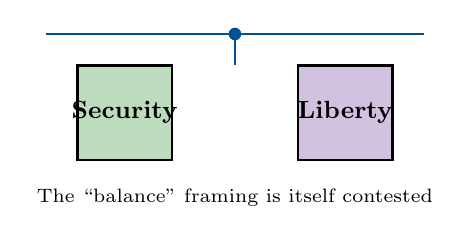
\begin{tikzpicture}[scale=0.8]
    % Balance beam
    \draw[thick, privacyblue] (-3,0) -- (3,0);
    \draw[thick, privacyblue] (0,-0.5) -- (0,0);
    \fill[privacyblue] (0,0) circle (0.1);
    
    % Left side - Security
    \draw[thick, fill=privacygreen!30] (-2.5,-0.5) rectangle (-1,-2);
    \node[font=\small\bfseries] at (-1.75,-1.25) {Security};
    
    % Right side - Liberty
    \draw[thick, fill=privacypurple!30] (1,-0.5) rectangle (2.5,-2);
    \node[font=\small\bfseries] at (1.75,-1.25) {Liberty};
    
    \node[below, font=\scriptsize] at (0,-2.3) {The ``balance'' framing is itself contested};
\end{tikzpicture}
\end{center}

\vspace{0.3em}
\textbf{Traditional framing}: Security vs. Liberty tradeoff

\textbf{Alternative framing}: False dichotomy---privacy \emph{enables} security (from abuse of power)

\textbf{Question}: How do we evaluate surveillance in democracies?
\end{frame}

% Slide 33: Arguments FOR Surveillance - Overview
\begin{frame}{The Case FOR Surveillance}
\begin{probox}[Core Claims]
\small
Proponents argue surveillance is necessary for security, justice, and public safety:
\begin{itemize}
    \item Surveillance deters crime through visibility.
    \item Surveillance helps solve crimes by providing evidence for prosecution.
    \item Surveillance can prevent terrorism by identifying threats before attacks.
    \item Public spaces carry no reasonable expectation of privacy anyway.
\end{itemize}
\end{probox}

\vspace{0.3em}
Let's examine one of these arguments more carefully...
\end{frame}

% Slide 34: The Deterrence Argument in Standard Form
\begin{frame}{The Deterrence Argument (Standard Form)}
\begin{probox}[Argument for Surveillance]
\small
\begin{enumerate}
    \item Deterring crime protects public safety, a legitimate government interest.
    \item Surveillance deters crime: people behave better when they know they're watched.
    \item If surveillance deters crime and deterring crime is legitimate, then surveillance is justified.
    \item Therefore, surveillance is justified.
\end{enumerate}
\end{probox}

\vspace{0.1em}
\begin{objectionbox}[Critique]
\scriptsize
\textbf{Premise 2 is empirically weak}: Studies on CCTV show mixed results. A 2019 meta-analysis found cameras reduce vehicle crime in parking lots but show ``no significant effect'' on violent crime.

\textbf{Premise 3 assumes proportionality}: Even if surveillance provides \emph{some} benefit, the argument doesn't show the benefit outweighs the costs (chilling effects, mission creep, abuse potential).
\end{objectionbox}
\end{frame}

% Slide 35: Arguments AGAINST Surveillance - Overview
\begin{frame}{The Case AGAINST Surveillance}
\begin{objectionbox}[Core Claims]
\small
Critics argue surveillance threatens liberty, equality, and democracy:
\begin{itemize}
    \item Surveillance creates chilling effects---people self-censor when watched.
    \item Surveillance creates dangerous power asymmetries between state and citizen.
    \item Surveillance systems inevitably expand beyond their original purpose.
    \item Surveillance technologies encode and amplify existing biases.
\end{itemize}
\end{objectionbox}

\vspace{0.3em}
Let's examine one of these arguments more carefully...
\end{frame}

% Slide 36: The Chilling Effects Argument in Standard Form
\begin{frame}{The Chilling Effects Argument (Standard Form)}
\begin{objectionbox}[Argument Against Surveillance]
\scriptsize
\begin{enumerate}
    \item A free society requires citizens can speak, associate, and explore ideas without fear.
    \item When people know they're watched, they self-censor---avoiding controversial speech, associations, and searches, even legal ones.
    \item Mass surveillance means people are (or believe they are) always watched.
    \item Therefore, mass surveillance undermines the conditions necessary for a free society.
\end{enumerate}
\end{objectionbox}

\vspace{0.05em}
\begin{probox}[Response]
\scriptsize
\textbf{Empirical challenge}: Do chilling effects occur at scale? Post-Snowden studies found measurable decreases in terrorism-related searches, suggesting the effect is real.

\textbf{Targeting response}: Supporters argue \emph{targeted} surveillance (with warrants) avoids mass chilling effects while preserving security benefits.
\end{probox}
\end{frame}

% Slide 37: The Nothing to Hide Argument Examined
\begin{frame}{The ``Nothing to Hide'' Argument (Standard Form)}
\begin{probox}[The Argument]
\scriptsize
\begin{enumerate}
    \item Surveillance only harms people who have something to hide.
    \item Law-abiding citizens have nothing to hide.
    \item Therefore, law-abiding citizens are not harmed by surveillance.
    \item Therefore, law-abiding citizens should not oppose surveillance.
\end{enumerate}
\end{probox}

\begin{objectionbox}[Multiple Problems]
\scriptsize
\begin{itemize}
    \item \textbf{Premise 1 is false}: Surveillance harms through chilling effects, power imbalances, errors, and abuse---none requiring wrongdoing.
    \item \textbf{Premise 2 is misleading}: Everyone has \emph{something} to hide---legal but private matters. ``Nothing to hide'' conflates privacy with guilt.
    \item \textbf{Ignores aggregation}: Innocuous data points combine into sensitive profiles.
    \item \textbf{Assumes static law}: Today's legal behavior may be tomorrow's crime.
\end{itemize}
\end{objectionbox}
\end{frame}

% Slide 38: Facial Recognition Debate
\begin{frame}{Facial Recognition---The Debate}
\begin{columns}[T]
\begin{column}{0.48\textwidth}
\begin{probox}[Pro Arguments]
\small
\begin{itemize}
    \item Identifies suspects, missing persons
    \item Faster than manual review
    \item Real-time response capability
\end{itemize}
\end{probox}
\end{column}
\begin{column}{0.48\textwidth}
\begin{objectionbox}[Con Arguments]
\small
\begin{itemize}
    \item Higher error rates for darker skin, women
    \item Face is public---permanent ID
    \item Chilling effect on protest
    \item No consent mechanism
\end{itemize}
\end{objectionbox}
\end{column}
\end{columns}

\vspace{0.3em}
\textbf{ACLU study}: 28 members of Congress falsely matched to mugshots

\textbf{Status}: Bans in San Francisco (2019, first US city), Boston, Oakland, 16+ municipalities
\end{frame}

% Slide 39: Clearview AI
\begin{frame}{Case Study: Clearview AI}
\begin{casestudybox}[The Controversial Facial Recognition Company]
\small
\textbf{Database}: Scraped \textbf{30+ billion photos} from social media (CEO claims 50B)\\
\textbf{Product}: App for police to identify anyone from a photo\\
\textbf{Customers}: 2,400+ law enforcement agencies (often without official approval)
\end{casestudybox}

\vspace{0.2em}
\textbf{Legal battles}:
\begin{itemize}
    \item Sued by ACLU; settled with ban on sales to private businesses
    \item Fined \texteuro30.5M (Netherlands), \texteuro20M (Italy), \pounds7.5M (UK)
    \item Banned in Australia, Canada
\end{itemize}

\textbf{CEO claim}: ``First Amendment right'' to collect public photos

\begin{alertblock}{Discussion}
Should police be able to identify anyone, anywhere, anytime?
\end{alertblock}
\end{frame}

% Slide 40: Predictive Policing
\begin{frame}{Predictive Policing}
\begin{conceptbox}[Using Data to Predict Crime]
\small
\textbf{Place-based}: Predict crime hotspots (PredPol, HunchLab)\\
\textbf{Person-based}: Predict who will commit/be victim of crime (Chicago ``heat list'')
\end{conceptbox}

\vspace{0.3em}
\textbf{Criticisms}:
\begin{itemize}
    \item \textbf{Feedback loops} emerge: police go where predicted $\rightarrow$ more arrests $\rightarrow$ more predictions for that area.
    \item Systems trained on historically biased enforcement data reproduce that bias.
    \item The \textbf{pre-crime problem}: are we punishing predicted future acts?
    \item Proprietary algorithms can't be challenged in court---an \textbf{opacity} problem.
    \item Limited evidence these systems actually reduce crime.
\end{itemize}

\textbf{Case}: Los Angeles ended PredPol (2020) after bias concerns
\end{frame}

% Slide 41: Workplace Surveillance
\begin{frame}{Workplace and Consumer Surveillance}
\begin{columns}[T]
\begin{column}{0.48\textwidth}
\textbf{Workplace monitoring}:
\begin{itemize}
    \item Keystroke logging, screenshots
    \item Productivity scoring
    \item Location tracking
    \item Amazon ``time off task''
    \item Remote work: Webcam, mouse tracking
\end{itemize}

\textbf{Stats}: 80\% of major companies monitor employees
\end{column}
\begin{column}{0.48\textwidth}
\textbf{Consumer surveillance}:
\begin{itemize}
    \item Smart home devices (Alexa recordings reviewed by humans)
    \item Connected cars (location, driving)
    \item Insurance apps (health tracking)
    \item Retail facial recognition
\end{itemize}
\end{column}
\end{columns}

\vspace{0.3em}
\textbf{Key point}: Government isn't the only surveillor---private companies too
\end{frame}

% Slide 42: Sophisticated Response to Nothing to Hide
\begin{frame}{The ``Nothing to Fear'' Response---Revisited}
\begin{objectionbox}[Sophisticated Responses to Surveillance]
\small
\begin{enumerate}
    \item \textbf{Definitional problem}: Who decides what's ``wrong''? Laws change.
    \item Information appropriate in one context isn't in another---\textbf{contextual integrity}.
    \item Innocuous data points combine into sensitive profiles---\textbf{aggregation}.
    \item Even innocent people change behavior when watched---\textbf{chilling effects}.
    \item Surveillance creates \textbf{power asymmetry}: ``Show me yours first.''
    \item Surveillance falls disproportionately on marginalized groups---\textbf{equality}.
\end{enumerate}
\end{objectionbox}

\vspace{0.1em}
\textbf{Bruce Schneier}: ``Too many wrongly characterize the debate as `security versus privacy.' The real choice is liberty versus control.''
\end{frame}

% Slide 43: Frameworks for Democratic Surveillance
\begin{frame}{Possible Frameworks for Democratic Surveillance}
\begin{conceptbox}[Constraints for Democratic Surveillance]
\small
\begin{enumerate}
    \item Warrants should be required with meaningful \textbf{judicial oversight}.
    \item The public should know what systems exist---\textbf{transparency}.
    \item Data should only be used for specified purposes---\textbf{purpose limitation}.
    \item Collect only what's necessary---the principle of \textbf{minimization}.
    \item Data should be deleted after a set period---\textbf{retention limits}.
    \item Record who accesses what data---\textbf{audit trails}.
    \item There must be real consequences for misuse---\textbf{accountability}.
    \item Programs should expire without reauthorization---\textbf{sunset clauses}.
\end{enumerate}
\end{conceptbox}
\end{frame}

% Slide 44: Key Tensions
\begin{frame}{Privacy in the Balance---Key Tensions}
\begin{center}
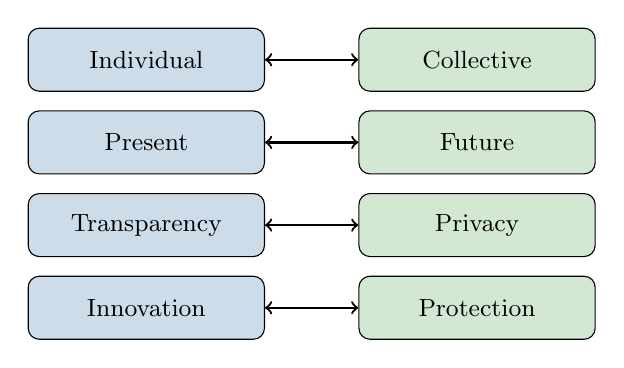
\begin{tikzpicture}[scale=0.7, every node/.style={font=\small}]
    % Four tension pairs
    \node[draw, rounded corners, fill=privacyblue!20, minimum width=3cm, minimum height=0.8cm] (ind) at (-3,2) {Individual};
    \node[draw, rounded corners, fill=privacygreen!20, minimum width=3cm, minimum height=0.8cm] (col) at (3,2) {Collective};
    \draw[<->, thick] (ind) -- (col);
    
    \node[draw, rounded corners, fill=privacyblue!20, minimum width=3cm, minimum height=0.8cm] (pre) at (-3,0.5) {Present};
    \node[draw, rounded corners, fill=privacygreen!20, minimum width=3cm, minimum height=0.8cm] (fut) at (3,0.5) {Future};
    \draw[<->, thick] (pre) -- (fut);
    
    \node[draw, rounded corners, fill=privacyblue!20, minimum width=3cm, minimum height=0.8cm] (trans) at (-3,-1) {Transparency};
    \node[draw, rounded corners, fill=privacygreen!20, minimum width=3cm, minimum height=0.8cm] (priv) at (3,-1) {Privacy};
    \draw[<->, thick] (trans) -- (priv);
    
    \node[draw, rounded corners, fill=privacyblue!20, minimum width=3cm, minimum height=0.8cm] (inn) at (-3,-2.5) {Innovation};
    \node[draw, rounded corners, fill=privacygreen!20, minimum width=3cm, minimum height=0.8cm] (prot) at (3,-2.5) {Protection};
    \draw[<->, thick] (inn) -- (prot);
\end{tikzpicture}
\end{center}

\vspace{0.2em}
These tensions cannot be fully ``resolved''---they must be navigated case by case.
\end{frame}

% Slide 46: Conclusion
\begin{frame}{Conclusion: Framework for Evaluation}
\begin{conceptbox}[Questions to Ask About Any Surveillance System]
\small
\begin{enumerate}
    \item \textbf{Who benefits} from this surveillance?
    \item \textbf{Who bears} the risks and costs?
    \item What \textbf{oversight and accountability} exists?
    \item Is this the \textbf{least invasive means} to the goal?
    \item What happens \textbf{when (not if)} it's abused?
\end{enumerate}
\end{conceptbox}

\vspace{0.3em}
\begin{alertblock}{Final Discussion}
Where do you draw the line? What surveillance, if any, is acceptable in a free society?
\end{alertblock}

\vspace{0.2em}
\textbf{Remember}: Privacy is not about having something to hide---it's about maintaining the boundaries that make us human.
\end{frame}

\end{document}